%%%%%%%% ICML 2026 EXAMPLE LATEX SUBMISSION FILE %%%%%%%%%%%%%%%%%

\documentclass{article}

% Recommended, but optional, packages for figures and better typesetting:
\usepackage{microtype}
\usepackage{graphicx}
\usepackage{subcaption}
\usepackage{booktabs} % for professional tables
\usepackage[normalem]{ulem}

\usepackage{tikz}
\usetikzlibrary{arrows.meta, positioning, shapes.geometric, fit, backgrounds, calc}

% hyperref makes hyperlinks in the resulting PDF.
% If your build breaks (sometimes temporarily if a hyperlink spans a page)
% please comment out the following usepackage line and replace
% \usepackage{icml2026} with \usepackage[nohyperref]{icml2026} above.
\usepackage{hyperref}


% Attempt to make hyperref and algorithmic work together better:
\newcommand{\theHalgorithm}{\arabic{algorithm}}

% Use the following line for the initial blind version submitted for review:
\usepackage{icml2026}

% For preprint, use
% \usepackage[preprint]{icml2026}

% If accepted, instead use the following line for the camera-ready submission:
% \usepackage[accepted]{icml2026}

\usepackage{amsmath}
\usepackage{amssymb}
\usepackage{mathtools}
\usepackage{amsthm}


% if you use cleveref..
\usepackage[capitalize,noabbrev]{cleveref}

%%%%%%%%%%%%%%%%%%%%%%%%%%%%%%%%
% THEOREMS
%%%%%%%%%%%%%%%%%%%%%%%%%%%%%%%%
\theoremstyle{plain}
\newtheorem{theorem}{Theorem}[section]
\newtheorem{proposition}[theorem]{Proposition}
\newtheorem{lemma}[theorem]{Lemma}
\newtheorem{corollary}[theorem]{Corollary}
\theoremstyle{definition}
\newtheorem{definition}[theorem]{Definition}
\newtheorem{assumption}[theorem]{Assumption}
\theoremstyle{remark}
\newtheorem{remark}[theorem]{Remark}

% Todonotes is useful during development; simply uncomment the next line
%    and comment out the line below the next line to turn off comments
%\usepackage[disable,textsize=tiny]{todonotes}
\usepackage[textsize=tiny]{todonotes}

% The \icmltitle you define below is probably too long as a header.
% Therefore, a short form for the running title is supplied here:
\icmltitlerunning{Submission and Formatting Instructions for ICML 2026}

\begin{document}

\twocolumn[
  \icmltitle{Progressive Cramming: Reliable Token Compression and What It Reveals}

  % It is OKAY to include author information, even for blind submissions: the
  % style file will automatically remove it for you unless you've provided
  % the [accepted] option to the icml2026 package.

  % List of affiliations: The first argument should be a (short) identifier you
  % will use later to specify author affiliations Academic affiliations
  % should list Department, University, City, Region, Country Industry
  % affiliations should list Company, City, Region, Country

  % You can specify symbols, otherwise they are numbered in order. Ideally, you
  % should not use this facility. Affiliations will be numbered in order of
  % appearance and this is the preferred way.
  \icmlsetsymbol{equal}{*}

  \begin{icmlauthorlist}
    \icmlauthor{Firstname1 Lastname1}{equal,yyy}
    \icmlauthor{Firstname2 Lastname2}{equal,yyy,comp}
    \icmlauthor{Firstname3 Lastname3}{comp}
    \icmlauthor{Firstname4 Lastname4}{sch}
    \icmlauthor{Firstname5 Lastname5}{yyy}
    \icmlauthor{Firstname6 Lastname6}{sch,yyy,comp}
    \icmlauthor{Firstname7 Lastname7}{comp}
    %\icmlauthor{}{sch}
    \icmlauthor{Firstname8 Lastname8}{sch}
    \icmlauthor{Firstname8 Lastname8}{yyy,comp}
    %\icmlauthor{}{sch}
    %\icmlauthor{}{sch}
  \end{icmlauthorlist}

  \icmlaffiliation{yyy}{Department of XXX, University of YYY, Location, Country}
  \icmlaffiliation{comp}{Company Name, Location, Country}
  \icmlaffiliation{sch}{School of ZZZ, Institute of WWW, Location, Country}

  \icmlcorrespondingauthor{Firstname1 Lastname1}{first1.last1@xxx.edu}
  \icmlcorrespondingauthor{Firstname2 Lastname2}{first2.last2@www.uk}

  % You may provide any keywords that you find helpful for describing your
  % paper; these are used to populate the "keywords" metadata in the PDF but
  % will not be shown in the document
  \icmlkeywords{Machine Learning, ICML}

  \vskip 0.3in
]

% this must go after the closing bracket ] following \twocolumn[ ...

% This command actually creates the footnote in the first column listing the
% affiliations and the copyright notice. The command takes one argument, which
% is text to display at the start of the footnote. The \icmlEqualContribution
% command is standard text for equal contribution. Remove it (just {}) if you
% do not need this facility.

% Use ONE of the following lines. DO NOT remove the command.
% If you have no special notice, KEEP empty braces:
\printAffiliationsAndNotice{}  % no special notice (required even if empty)
% Or, if applicable, use the standard equal contribution text:
% \printAffiliationsAndNotice{\icmlEqualContribution}

\begin{abstract}
    Token cramming compresses sequences into learned embeddings with near-perfect reconstruction, but prior work used fixed token budgets and 99\% accuracy thresholds -- leaving open whether residual errors reflect fundamental limits or optimization failures, and whether reconstruction implies useful compression. We introduce progressive cramming: sequentially adding tokens until 100\% accuracy, with two stabilizing techniques -- activation alignment and low-dimensional projection. This achieves reliable perfect reconstruction and enables precise measurement of per-model information gain. Analyzing optimization trajectories, we find they occupy surprisingly low-dimensional manifolds. Attention analysis reveals why optimization is difficult -- compression tokens hijack 40-80\% of attention mass in intermediate layers. However, evaluating compressed prefixes on HellaSwag and ARC exposes a fundamental limit: models fail entirely, even with decompressed tokens in context. Cramming achieves reconstruction by overriding model computation, not by encoding transferable semantics. Our results establish progressive cramming as a tool for studying compression limits while demonstrating that even perfect reconstruction is insufficient for meaningful compression
\end{abstract}


\section{Introduction}
\label{sec:introduction}

How much information can a single embedding encode?
Recent work on ``cramming'' \cite{kuratov2025cramming} probed this question by optimizing embeddings to reconstruct token sequences through autoregressive decoding.
The results were striking: single embeddings in the input space of large language models can encode up to 1568  tokens with near-perfect reconstruction accuracy, suggesting enormous latent capacity in transformer representations.

% PARAGRAPH 2: The open question - HOW does it work?
But \emph{how} do transformers achieve this?
The original work focused on capacity limits -- how many tokens fit -- rather than the mechanism enabling reconstruction.
This leaves open a fundamental question: does cramming discover dense semantic representations that the model can interpret, or does it exploit some other property of transformer computation?
Understanding this mechanism matters beyond cramming itself; it reveals how transformers process information stored in their embedding space.

% PARAGRAPH 3: Methodological improvements enabling study
We first address methodological limitations that complicate controlled study.
Prior work used fixed token budgets and 99\% accuracy thresholds with teacher forcing. But the last 1\% of errors may lead to catastrophic failures in autoregressive generation without teacher forcing.
We introduce \emph{progressive cramming}: sequentially adding tokens until perfect reconstruction, with two stabilizing techniques -- activation alignment and low-dimensional projection.
This achieves reliable 100\% accuracy and enables precise measurement of where compression fails.

% PARAGRAPH 4: What we find - the mechanism
With these tools, we investigate the cramming mechanism.
Analysis of optimization trajectories reveals they occupy surprisingly low-dimensional manifolds: 30-100 PCA components explain 99\% of variance in 2048-4096 dimensional embedding spaces.
More critically, attention pattern analysis exposes \emph{how} reconstruction occurs: compression embeddings hijack 40-80\% of attention mass in intermediate layers.
This concentration is invariant to sequence length -- the same layers are dominated whether cramming 32 or 512 tokens -- suggesting compression activates fixed circuits rather than scaling information density.

% PARAGRAPH 5: What this means - not semantic encoding
This mechanism has consequences.
If cramming worked through semantic encoding, compressed prefixes should preserve downstream capabilities.
Evaluation on HellaSwag and ARC reveals the opposite: models fail entirely, even when decompressed tokens remain in context.
Cramming achieves reconstruction by \emph{overriding} transformer computation -- forcing specific outputs through attention capture -- rather than by encoding information the model can flexibly use.

% PARAGRAPH 6: Implications
These findings reframe what cramming reveals about transformers.
The high capacity demonstrated by prior work reflects not dense semantic encoding but the ease of hijacking attention mechanisms.
This distinction matters for future work on learned compression: methods that override computation can achieve perfect reconstruction while encoding nothing transferable.

Our main contributions are follows:
\begin{itemize}
    \item Progressive cramming framework with activation alignment and low-dimensional projection, achieving reliable 100\% reconstruction
    \item Analysis revealing optimization trajectories occupy low-dimensional manifolds
    \item Discovery that cramming works through attention hijacking: compression tokens capture 40-80\% of attention mass in fixed intermediate layers
    \item Demonstration that this mechanism fails to preserve downstream capabilities, distinguishing reconstruction from semantic encoding
\end{itemize}



% =============================================================================
\section{Related Work}
\label{sec:related_work}
% =============================================================================


\subsection{Token Cramming}

Our work is primarily built upon the token cramming framework introduced by \citet{kuratov2025cramming}, who demonstrate that per-sample optimization can compress up to 1,568 tokens into a single input embedding of Llama-3.1-8B, achieving compression ratios of approximately $1500\times$ -- two orders of magnitude beyond encoder-based approaches that typically achieve at most $10\times$ lossless compression. Their work reveals a substantial gap between the theoretical information capacity of high-dimensional embedding spaces and what current methods practically achieve. Crucially, they show that compression capacity is determined primarily by the cross-entropy reduction rather than raw sequence length, suggesting that the model leverages its internalized knowledge to complement the information stored in the embedding.

Extending this line of inquiry, \citet{mezentsev2025exploring} investigate whether autoregressive decoding is essential for reconstruction from compressed embeddings. They demonstrate that frozen LLMs can generate hundreds of accurate tokens in a single forward pass in non-autoregressive way when provided with just two learned ``proto-token'' embeddings, revealing an underexplored multi-token generation capability. Their analysis shows that valid compression representations form connected, local regions in embedding space rather than isolated points, suggesting the potential for learning practical encoders.


\subsection{Context Compression and Distillation}

A parallel line of research addresses context compression for the purpose of reducing computational costs during inference. Importantly, these approaches differ fundamentally from token cramming in their objective: they focus on \emph{semantic compression} that preserves task-relevant information for downstream use, rather than \emph{exact reconstruction} of the original token sequence.

\citet{zhang2025activations_beacon} propose Activation Beacon, a plug-in module that compresses the keys and values at every transformer layer into special beacon tokens. By directly compressing activations rather than relying on soft prompts to relay information, their method achieves flexible compression ratios while preserving the LLM's capabilities on short contexts. The progressive, chunk-wise compression workflow enables processing of contexts up to 400K tokens.

\citet{chevalier-etal-2023-autocompressors} adapt pre-trained language models into AutoCompressors that learn to compress long contexts into compact summary vectors through an unsupervised objective. These summary vectors function as soft prompts, enabling the model to condition on compressed representations of previous segments during language modeling. Their approach processes documents in segments, accumulating summary information across the sequence.

The In-context Autoencoder (ICAE) of \citet{ge2024ICAE} employs a LoRA-adapted encoder to compress contexts into memory slots that the target LLM can condition upon. Pre-trained with both autoencoding and language modeling objectives, ICAE achieves $4\times$ context compression while maintaining the ability to respond to various prompts. The method draws interesting parallels between working memory in cognitive science and context representation in LLMs.

These semantic compression methods are designed to preserve information relevant for downstream tasks such as question answering or summarization, tolerating lossy compression of details not essential for the target application. In contrast, our work and the cramming literature focus on near-lossless reconstruction, which provides a cleaner setting for studying the fundamental capacity and mechanisms of embedding-based information storage.

\subsection{Soft Prompts and Prefix Tuning}

The optimization of continuous embeddings as model inputs originated in parameter-efficient fine-tuning research. \citet{li-liang-2021-prefix-tuning} introduce prefix-tuning, which prepends learnable continuous vectors to the input that subsequent tokens can attend to as ``virtual tokens.'' By optimizing only $0.1\%$ of parameters while keeping the language model frozen, prefix-tuning achieves comparable performance to full fine-tuning on generation tasks while enabling efficient multi-task deployment.

\citet{lester-etal-2021-prompt-tuning} propose prompt tuning, a simplified approach that learns soft prompts only at the input layer rather than at every transformer layer. They demonstrate that prompt tuning becomes increasingly competitive with full model tuning as model scale increases, with billion-parameter models closing the gap entirely. This finding suggests that larger models develop embedding spaces with sufficient structure to support rich task-specific conditioning through input manipulation alone.

These methods establish that frozen language models can be effectively steered through learned embeddings without modifying model parameters. Token cramming can be viewed as an extreme case of this paradigm: rather than encoding task-specific instructions, the learned embedding must encode the complete information content of an arbitrary token sequence. Our progressive cramming methodology bridges these perspectives by studying how compression tokens interact with the model's attention and activation patterns as the encoding task becomes increasingly demanding.

\paragraph{Mechanistic Interpretability.}

{\color{red} TODO? Logit lens, activation patching, attention analysis. Methods we use for understanding hijacking.}


% =============================================================================
\section{Background: Token Cramming}
\label{sec:background}
% =============================================================================

\subsection{Problem Formulation}

In the cramming task, a single embedding is optimized to encode as many tokens as possible through autoregressive reconstruction. The language model weights remain frozen throughout optimization, and each sequence receives a newly initialized compression embedding.

Let $\mathcal{M}$ be an autoregressive language model with vocabulary $\mathcal{V}$ and embedding dimension $d$.
Given a target sequence $\mathbf{x} = (x_1, \ldots, x_n)$ where $x_i \in \mathcal{V}$, the cramming objective finds an embedding $\mathbf{e} \in \mathbb{R}^d$ such that:
%
\begin{equation}
    \mathbf{e}^* = \arg\min_{\mathbf{e}} \mathcal{L}_{\text{cram}}(\mathbf{e}; \mathbf{x}, \mathcal{M})
\end{equation}
%
where the cramming loss is the cross-entropy over the target sequence:
%
\begin{equation}
    \mathcal{L}_{\text{cram}}(\mathbf{e}; \mathbf{x}, \mathcal{M}) = -\sum_{i=1}^{n} \log p_{\mathcal{M}}(x_i \mid \mathbf{e}, x_1, \ldots, x_{i-1})
\end{equation}

\subsection{Limitations of Prior Work}\label{sec:prior_limitations}

{\color{red}
    Describe 99\% threshold and fixed token budget limitations. Cite specific numbers from original paper.

    The Last 1\% Problem. Show example of how 1 early error cascades in autoregressive decoding. Most errors are happen at firs two tokens for full cramming.

    Fixed Budget Obscures Limits. Explain why fixed token counts don't reveal true information-theoretic limits.
}



% =============================================================================
\section{Method: Progressive Cramming}
\label{sec:method}
% =============================================================================

\subsection{Progressive Token Addition}
\label{sec:progressive}

Rather than optimizing a compression embedding for a fixed-length target, we progressively extend the target prefix and warm-start optimization:
%
\begin{enumerate}
    \item Initialize with $\mathbf{x}^{(1)} = (x_1)$ and optimize $\mathbf{e}^{(1)} \in \mathbb{R}^d$ until perfect reconstruction.
    \item Extend to $\mathbf{x}^{(k)} = (x_1, \ldots, x_k)$, initialize $\mathbf{e}^{(k)} \leftarrow \mathbf{e}^{(k-1)}$, and continue optimizing for the longer prefix.
    \item Repeat until perfect reconstruction is no longer achievable within the optimization budget.
\end{enumerate}

This process is visualized on Figure~\ref{fig:progressive}.

Progressive cramming produces a sequence of embeddings $\{\mathbf{e}^{(k)}\}_{k=1}^{n}$, where $\mathbf{e}^{(k)}$ is the optimized compression embedding for the length-$k$ prefix.
This lets us quantify how far the optimizer moves in embedding space as new tokens are added.
We define the (stage-wise) trajectory length as the sum of Euclidean distances between consecutive stages:

\begin{equation}
    L_{\text{traj}} = \sum_{k=1}^{n-1} \left\| \mathbf{e}^{(k+1)} - \mathbf{e}^{(k)} \right\|_2
\end{equation}



\begin{figure*}[t]
    \centering
    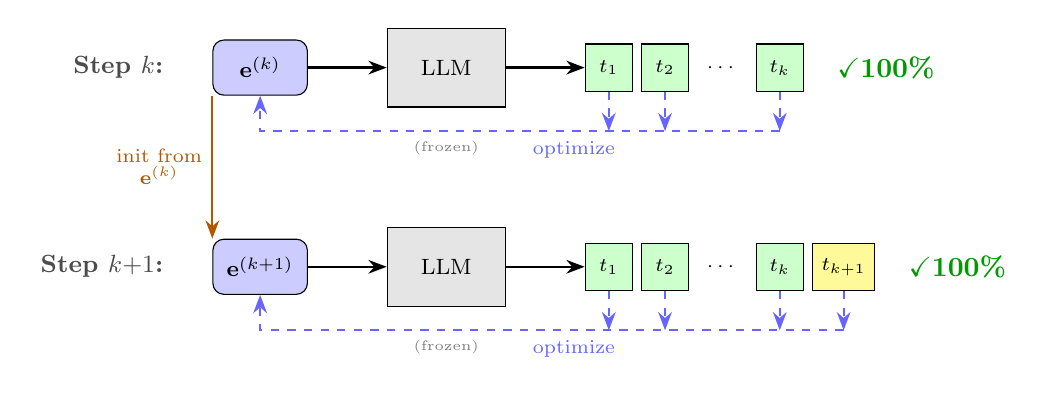
\begin{tikzpicture}[
    >=Stealth,
    node distance=0.8cm,
    emb/.style={draw, rounded corners, fill=blue!20, minimum width=1.2cm, minimum height=0.7cm, font=\footnotesize},
    llm/.style={draw, fill=gray!20, minimum width=1.5cm, minimum height=1cm, font=\footnotesize},
    token/.style={draw, fill=green!20, minimum width=0.6cm, minimum height=0.6cm, font=\scriptsize},
    check/.style={text=green!60!black, font=\bfseries},
    stage/.style={font=\small\bfseries, text=black!70},
    optim/.style={->, thick, blue!60, dashed},
    init/.style={->, thick, orange!70!black},
]

% === STAGE k ===
\node[stage] (stage1) {\makebox[1.5cm][r]{Step $k$}:};

\node[emb, right=0.5cm of stage1] (e1) {$\mathbf{e}^{(k)}$};
\node[llm, right=1cm of e1] (llm1) {LLM};
\node[token, right=1cm of llm1] (t1_1) {$t_1$};
\node[token, right=0.1cm of t1_1] (t1_2) {$t_2$};
\node[right=0.1cm of t1_2, font=\scriptsize] (dots1) {$\cdots$};
\node[token, right=0.1cm of dots1] (t1_k) {$t_k$};

% Arrows for stage k
\draw[->, thick] (e1) -- (llm1);
\draw[->, thick] (llm1) -- (t1_1);

% Checkmark
\node[check, right=0.3cm of t1_k] (check1) {\checkmark 100\%};

% Optimization loop for stage k - spans all tokens
\coordinate (loop1_right) at ($(t1_k.south) + (0, -0.5)$);
\coordinate (loop1_left) at ($(t1_1.south) + (0, -0.5)$);
\draw[optim] (t1_1.south) -- (loop1_left);
\draw[optim] (t1_2.south) -- ++(0, -0.5);
\draw[optim] (t1_k.south) -- (loop1_right);
\draw[optim] (loop1_right) -- (loop1_left) -| node[pos=0.05, below, font=\scriptsize, text=blue!60] {optimize} (e1.south);

% === STAGE k+1 ===
\node[stage, below=2cm of stage1] (stage2) {\makebox[1.5cm][r]{Step $k{+}1$}:};

\node[emb, right=0.5cm of stage2] (e2) {$\mathbf{e}^{(k+1)}$};
\node[llm, right=1cm of e2] (llm2) {LLM};
\node[token, right=1cm of llm2] (t2_1) {$t_1$};
\node[token, right=0.1cm of t2_1] (t2_2) {$t_2$};
\node[right=0.1cm of t2_2, font=\scriptsize] (dots2) {$\cdots$};
\node[token, right=0.1cm of dots2] (t2_k) {$t_k$};
\node[token, right=0.1cm of t2_k, fill=yellow!40] (t2_k1) {$t_{k+1}$};

% Arrows for stage k+1
\draw[->, thick] (e2) -- (llm2);
\draw[->, thick] (llm2) -- (t2_1);

% Checkmark
\node[check, right=0.3cm of t2_k1] (check2) {\checkmark 100\%};

% Optimization loop for stage k+1 - spans all tokens
\coordinate (loop2_right) at ($(t2_k1.south) + (0, -0.5)$);
\coordinate (loop2_left) at ($(t2_1.south) + (0, -0.5)$);
\draw[optim] (t2_1.south) -- (loop2_left);
\draw[optim] (t2_2.south) -- ++(0, -0.5);
\draw[optim] (t2_k.south) -- ++(0, -0.5);
\draw[optim] (t2_k1.south) -- (loop2_right);
\draw[optim] (loop2_right) -- (loop2_left) -| node[pos=0.05, below, font=\scriptsize, text=blue!60] {optimize} (e2.south);

% === INITIALIZATION ARROW ===
\draw[init] (e1.south west) -- (e2.north west)
    node[midway, left, font=\scriptsize, text=orange!70!black, align=center] {init from\\$\mathbf{e}^{(k)}$};

% === LABELS ===
\node[below=0.3cm of llm1, font=\tiny, text=gray] {(frozen)};
\node[below=0.3cm of llm2, font=\tiny, text=gray] {(frozen)};

\end{tikzpicture}
    \caption{Progressive cramming adds target tokens sequentially. At stage $k$, we optimize the compression representation to achieve 100\% reconstruction of the prefix $(x_1,\ldots,x_k)$, then extend to $k{+}1$ and warm-start from the previous solution.}
    \label{fig:progressive}
\end{figure*}

\subsection{Activation Alignment}
\label{sec:activation_alignment}

To stabilize optimization, we regularize hidden states toward those of the uncompressed sequence.
Let $\mathbf{h}_l^{\text{cram}}(i)$ denote the hidden state at layer $l$ and token position $i$ when the model is conditioned on the compression embedding, and let $\mathbf{h}_l^{\text{clean}}(i)$ be the corresponding state for the same token position without compression.
We align activations using cosine distance:
%
\begin{equation}
    \mathcal{L}_{\text{align}} = \frac{1}{n} \sum_{l \in \{1..K\}} \sum_{i=1}^{n} \left( 1 - \frac{\mathbf{h}_l^{\text{cram}}(i) \cdot \mathbf{h}_l^{\text{clean}}(i)}{\|\mathbf{h}_l^{\text{cram}}(i)\| \, \|\mathbf{h}_l^{\text{clean}}(i)\|} \right)
\end{equation}
%

where $K$ is the number of layers used for alignment.

The full objective combines reconstruction and alignment:

\begin{equation}
    \mathcal{L} = \mathcal{L}_{\text{cram}} + \alpha \mathcal{L}_{\text{align}}
\end{equation}

where $\alpha$ controls alignment strength.


\subsection{Low-Dimensional Projection}
\label{sec:lowdim}

We observed that optimization trajectories occupy low-dimensional subspaces (Section~\ref{sec:trajectory}).
This motivates constraining optimization to a learned projection:

\begin{equation}
    \mathbf{e} = \mathbf{W} \mathbf{z} + \mathbf{b}
\end{equation}

where $\mathbf{z} \in \mathbb{R}^k$ with $k \ll d$, $\mathbf{W} \in \mathbb{R}^{d \times k}$, and $\mathbf{b} \in \mathbb{R}^d$.
For each sample, we randomly initialize $(\mathbf{W}, \mathbf{b}, \mathbf{z})$ and optimize them jointly, which restricts the compression embedding to a rank-$k$ affine subspace.

After optimization, the effective embedding $\mathbf{e}$ can be materialized once and reused; the projection primarily changes the optimization geometry by introducing optimizer state (e.g., momentum) in the low-dimensional coordinates.

\subsection{Attention Mass}
\label{sec:attention_mass}

To quantify attention hijacking (Section~\ref{sec:attention}), we measure how much attention mass other positions allocate to the first position (position $0$), which corresponds to \texttt{[mem]} in crammed inputs or the BOS token in the uncompressed baseline.
Let $\mathbf{A}_l \in [0,1]^{S \times S}$ denote the attention matrix at layer $l$ after averaging over heads.
For a given prefix length $s \le S$, we define the attention mass on position $0$ as
%
\begin{equation}
    m_l(s) = \frac{1}{s-1} \sum_{q=1}^{s-1} \mathbf{A}_l(q, 0)
\end{equation}
%
which excludes self-attention ($q=0$) and averages over query positions.
We report $100 \cdot m_l(s)$ as a percentage, and average over a set of target prefix lengths $\mathcal{S}$:
%
\begin{equation}
    \bar{m}_l = \frac{1}{|\mathcal{S}|} \sum_{s \in \mathcal{S}} m_l(s)
\end{equation}

\subsection{Information Gain}

As a primary cramming metric we use information gain \cite{kuratov2025cramming}, defined as the reduction in total cross-entropy (in bits) on the target sequence when conditioning on the learned compression embedding.
Let $H_{LM}$ be the sum of per-token cross-entropies for the original token sequence, and let $H_{[mem]+LM}$ be the corresponding quantity when the model is conditioned on \texttt{[mem]}.

\begin{equation}
    C_H = H_{LM} - H_{[mem]+LM}
\end{equation}

\citet{kuratov2025cramming} show that cramming capacity is better characterized by information gain than by raw token count, and that this quantity is relatively stable across datasets.

% =============================================================================
\section{Experiments}
\label{sec:experiments}
% =============================================================================

We evaluate progressive cramming on PG19 \cite{Rae2020CompressiveTransformerPG19} across four model families: Pythia \cite{biderman2023pythia}, Llama~3 \cite{dubey2024llama3}, SmolLM2 \cite{allal2025smollm2}, and Gemma~3 \cite{gemma3}.
Unless stated otherwise, results report mean $\pm$ standard deviation over samples.

Table~\ref{tab:full_vs_progressive} compares progressive cramming (targeting 100\% reconstruction) to ``full'' cramming baselines that use fixed token budgets and may terminate below perfect accuracy.
Because autoregressive decoding is brittle to early errors (Section~\ref{sec:prior_limitations}), this comparison should be interpreted primarily through the lens of \emph{perfect} reconstruction: progressive cramming trades a fixed-budget constraint for a fixed-accuracy constraint, yielding different operating points in token count and information gain.

\begin{table}[]
    \centering
    \caption{Full vs. progressive cramming on PG19. ``Full'' cramming uses a fixed token budget and may stop below perfect reconstruction \cite{kuratov2025cramming}; progressive cramming fixes reconstruction at 100\% and reports the achieved token count.}\label{tab:full_vs_progressive}

\begin{tabular}{llll}
\hline
 Type                                           & Tokens                  & Info Gain                & Accuracy                   \\
\hline
 \multicolumn{4}{l}{\textbf{Llama-3.2-1B}} \\
 Full                                           & 256                     & 1028 {\small $\pm$ 163}  & 0.996 {\small $\pm$ 0}     \\
 Full                                           & 512                     & 1965 {\small $\pm$ 244}  & 0.998 {\small $\pm$ 0}     \\
 Progr.                                         & 402 {\small $\pm$ 85}   & 1500 {\small $\pm$ 282}  & 1.0                        \\
 \midrule
 \multicolumn{4}{l}{\textbf{Llama-3.2-3B}} \\
 Full                                           & 512                     & 1803 {\small $\pm$ 238}  & 0.999 {\small $\pm$ 0.001} \\
 Full                                           & 1024                    & 3572 {\small $\pm$ 549}  & 0.996 {\small $\pm$ 0.007} \\
 Progr.                                         & 902 {\small $\pm$ 207}  & 3074 {\small $\pm$ 527}  & 1.0                        \\
 \midrule
 \multicolumn{4}{l}{\textbf{Llama-3.1-8B}} \\
  Full                                           & 1024                    & 3316 {\small $\pm$ 581}  & 0.999 {\small $\pm$ 0.001} \\
 Full                                           & 1568                    & 5002 {\small $\pm$ 850}  & 0.997 {\small $\pm$ 0.003} \\
 Progr.                                         & 1064 {\small $\pm$ 394} & 3028 {\small $\pm$ 1321} & 1.0                        \\
 \midrule \midrule
 \multicolumn{4}{l}{\textbf{Pythia160m}} \\
 Full                                           & 32                      & 105 {\small $\pm$ 20}    & 0.684 {\small $\pm$ 0.175} \\
 Full                                           & 64                      & 130 {\small $\pm$ 20}    & 0.516 {\small $\pm$ 0.076} \\
 Progr.                                         & 11 {\small $\pm$ 2}     & 19 {\small $\pm$ 26}     & 1.0                        \\
 \midrule
 \multicolumn{4}{l}{\textbf{Pythia410m}} \\
 Full                                           & 96                      & 320 {\small $\pm$ 41}    & 0.959 {\small $\pm$ 0.031} \\
 Full                                           & 128                     & 365 {\small $\pm$ 40}    & 0.891 {\small $\pm$ 0.062} \\
 Progr.                                         & 102 {\small $\pm$ 41}   & 323 {\small $\pm$ 105}   & 1.0                        \\
 \midrule
 \multicolumn{4}{l}{\textbf{Pythia1.4b}} \\
 Full                                           & 128                     & 389 {\small $\pm$ 86}    & 1 {\small $\pm$ 0}         \\
 Full                                           & 256                     & 802 {\small $\pm$ 113}   & 0.985 {\small $\pm$ 0.031} \\
 Progr.                                         & 544 {\small $\pm$ 57}   & 1694 {\small $\pm$ 125}  & 1.0                        \\
\hline
\end{tabular}
    \label{tab:full_vs_progressive}
\end{table}


\subsection{Optimization Trajectories}
\label{sec:trajectory}

Progressive cramming enables tracking the optimization path through embedding space.
We record the sequence of optimized embeddings $\{\mathbf{e}^{(k)}\}_{k=1}^{n}$ and analyze its geometry.
Across model families, the trajectories are well-approximated by surprisingly low-dimensional structure: only a modest number of principal components explains 99\% of the trajectory variance, even when hundreds (or thousands) of tokens are reconstructed (Table~\ref{tab:pca_models}).

Figure~\ref{fig:pca_from_seq_length} shows that, for Llama-3.1-8B, the number of components required for 99\% variance grows sublinearly with prefix length and is consistent with a slow (approximately logarithmic) trend across learning rates.
Table~\ref{tab:pca_models} further highlights two qualitative patterns: (i) larger models tend to use more trajectory directions (higher PCA 99\%), and (ii) Gemma~3 achieves noticeably lower information gain at comparable or smaller token counts, consistent with optimization constraints induced by logits softcapping \cite{gemma2}.

{\color{red} TODO - reconstruction from PCA components}

{\color{red} TODO - shared subspaces?}
{\color{red} TODO visualize Optimization Landscape.}


\begin{table*}[]
    \centering
    \caption{Progressive cramming trajectory statistics on PG19. ``Compressed Tokens'' is the achieved prefix length $n$, ``Trajectory Length'' is $L_{\text{traj}}$, and ``PCA 99\%'' is the number of principal components explaining 99\% of trajectory variance.}
    \label{tab:pca_models}

\begin{tabular}{lllll}
\hline
 Model                         & Compressed Tokens           & Information Gain         & Trajectory Length        & PCA 99\%                   \\
\hline
 Llama-3.2-1B {\small lr=0.1}  & 402.2 {\small $\pm$ 84.8}   & 1500 {\small $\pm$ 282}  & 1736 {\small $\pm$ 206}  & 44.1 {\small $\pm$ 5.73}  \\
 Llama-3.2-3B {\small lr=0.1}  & 902.2 {\small $\pm$ 206.8}  & 3074 {\small $\pm$ 527}  & 4232 {\small $\pm$ 913}  & 61.5 {\small $\pm$ 4.54}  \\
 Llama-3.1-8B {\small lr=0.1}  & 1063.5 {\small $\pm$ 394.4} & 3028 {\small $\pm$ 1321} & 4861 {\small $\pm$ 1033} & 74.4 {\small $\pm$ 7.94}  \\
 \midrule
 pythia-160m {\small lr=0.5}   & 10.7 {\small $\pm$ 2}       & 19 {\small $\pm$ 26}     & 652 {\small $\pm$ 196}   & 5.1 {\small $\pm$ 1.64}   \\
 pythia-410m {\small lr=0.5}   & 102.1 {\small $\pm$ 40.8}   & 323 {\small $\pm$ 105}   & 3613 {\small $\pm$ 841}  & 37.5 {\small $\pm$ 11.16} \\
 pythia-1.4b {\small lr=0.5}   & 543.8 {\small $\pm$ 56.8}   & 1694 {\small $\pm$ 125}  & 6730 {\small $\pm$ 390}  & 49 {\small $\pm$ 3.32}    \\
 \midrule
 SmolLM2-135M {\small lr=0.1}  & 38.5 {\small $\pm$ 14.1}    & 168 {\small $\pm$ 66}    & 178 {\small $\pm$ 40}    & 12.2 {\small $\pm$ 2.96}  \\
 SmolLM2-360M {\small lr=0.1}  & 61 {\small $\pm$ 24.6}      & 266 {\small $\pm$ 122}   & 234 {\small $\pm$ 111}   & 13.4 {\small $\pm$ 3.95}  \\
 SmolLM2-1.7B {\small lr=0.1}  & 370.2 {\small $\pm$ 113.1}  & 1119 {\small $\pm$ 350}  & 1027 {\small $\pm$ 167}  & 29.2 {\small $\pm$ 2.93}  \\
 \midrule
 gemma-3-270m {\small lr=0.1}  & 71.2 {\small $\pm$ 14.2}    & 392 {\small $\pm$ 71}    & 259 {\small $\pm$ 32}    & 18.5 {\small $\pm$ 2.54}  \\
 gemma-3-1b-pt {\small lr=0.1} & 74.8 {\small $\pm$ 34.3}    & 338 {\small $\pm$ 104}   & 386 {\small $\pm$ 89}    & 18.9 {\small $\pm$ 6.59}  \\
 gemma-3-4b-pt {\small lr=0.1} & 286.5 {\small $\pm$ 164.6}  & 949 {\small $\pm$ 466}   & 1044 {\small $\pm$ 328}  & 31.8 {\small $\pm$ 9.21}  \\
\hline
\end{tabular}


\end{table*}


\begin{figure}[t]
    \centering
    \centerline{\includegraphics[width=\columnwidth]{aggregate_pca_components_vs_seq_len_Llama3.1-8B_all_lrs.pdf}}
    \caption{Number of principal components required to explain 99\% of progressive trajectory variance vs. reconstructed prefix length for Llama-3.1-8B, shown for multiple learning rates.}
    \label{fig:pca_from_seq_length}
\end{figure}

\subsection{Dataset Modifications}

To probe sensitivity to surface form, we create controlled variants of PG19 samples and compare their progressive trajectories (Figure~\ref{fig:trajectories_text_modifications}).
Each variant shares an identical 64-token prefix and modifies the suffix in one of three ways: random word permutation, greedy decoding from Llama-3.1-8B (``Sampled''), or lowercasing.
Trajectories coincide during the shared prefix and diverge immediately after the edit point, indicating that the optimization path is highly sensitive to token-level details.
Notably, lowercasing (which should preserve high-level semantics) induces a markedly different trajectory, suggesting that progressive cramming is driven by tokenization- and distribution-level properties rather than semantic equivalence.



\begin{figure*}[t]
    \centering
    \centerline{\includegraphics[width=\linewidth]{Llama3.1-8B-text-modifications_lr-0p1.pdf}}
    \caption{Progressive trajectories projected onto PCA components (Llama-3.1-8B, one PG19 sample). All variants share the same 64-token prefix; the suffix is either original (Base), randomly permuted (Random), greedily sampled continuation (Sampled), or lowercased (Lowercased). Circles mark the start and squares mark the end. Axis titles report the signed explained-variance fraction.}
    \label{fig:trajectories_text_modifications}
\end{figure*}



\begin{table}[]
    \centering
    \caption{Progressive cramming on modified PG19 samples (Llama-3.1-8B). All variants share a 64-token prefix and differ only in the suffix (Base/Random/Sampled/Lowercased). {\color{red} TODO recompute via \texttt{scripts/paper/text\_modifications\_table.py}.}}
    \label{tab:text_modifications}

\begin{tabular}{llll}
\hline
 Experiment   & Tokens                  & Info Gain                & PCA 99\%              \\
\hline
 Base         & 1048 {\small $\pm$ 404} & 3169 {\small $\pm$ 1212} & 74 {\small $\pm$ 8}  \\
 Random       & 1 {\small $\pm$ 0}      & 0 {\small $\pm$ 0}       & nan                  \\
 Sampled      & 2048 {\small $\pm$ 0}   & 432 {\small $\pm$ 141}   & 60 {\small $\pm$ 28} \\
 Lowercased   & 1 {\small $\pm$ 0}      & 0 {\small $\pm$ 0}       & nan                  \\
\hline
\end{tabular}


\end{table}

\subsection{Lowdim Projection}

Low-dimensional projection (Section~\ref{sec:lowdim}) changes the optimization geometry by restricting the learned embedding to an affine rank-$k$ subspace.
Empirically, this can improve stability and alter the effective capacity:
\begin{itemize}
    \item It often reduces sensitivity to learning rate by concentrating optimization into a smaller coordinate system.
    \item It can reduce the intrinsic dimensionality of trajectories (PCA 99\%) while preserving, or sometimes increasing, information gain.
\end{itemize}

Table~\ref{tab:low_dim_projection_results} ablates projection dimension across model families.
Three takeaways stand out:
\begin{itemize}
    \item For Llama-3.1-8B and SmolLM2-1.7B, projection can substantially increase achievable token counts and information gain compared to the unconstrained baseline.
    \item Increasing projection dimension does not reliably increase PCA 99\% (and can even decrease it), but it often increases the measured trajectory length, suggesting longer optimization paths within a similarly low-dimensional subspace.
    \item For Pythia-1.4B, small projection dimensions strongly reduce PCA 99\% and trajectory length, but also reduce capacity; adding a larger projection partially recovers information gain.
\end{itemize}

\begin{table*}[]
    \centering
    \caption{Effect of low-dimensional projection size on progressive cramming. ``dim'' in the model column denotes the projection dimension $k$ (Section~\ref{sec:lowdim}).}
    \label{tab:low_dim_projection_results}

\begin{tabular}{lllll}
\hline
 Model                         & Compressed Tokens           & Information Gain         & Trajectory Length         & PCA 99\%                  \\
\hline
 Llama-3.1-8B {\small lr=0.1}  & 1063.5 {\small $\pm$ 394.4} & 3028 {\small $\pm$ 1321} & 4861 {\small $\pm$ 1033}  & 74.4 {\small $\pm$ 7.94} \\
 Llama-3.1-8B {\small dim=32}  & 1745 {\small $\pm$ 306}     & 5312 {\small $\pm$ 330}  & 10250 {\small $\pm$ 3256} & 35.7 {\small $\pm$ 5.1}  \\
 Llama-3.1-8B {\small dim=256} & 1730.8 {\small $\pm$ 384.3} & 4870 {\small $\pm$ 1680} & 21448 {\small $\pm$ 5583} & 29.4 {\small $\pm$ 3.29} \\
 Llama-3.1-8B {\small dim=512} & 1652.9 {\small $\pm$ 404.5} & 5072 {\small $\pm$ 799}  & 25852 {\small $\pm$ 7528} & 36.2 {\small $\pm$ 5.88} \\
 \midrule
 pythia-1.4b {\small lr=0.5}   & 543.8 {\small $\pm$ 56.8}   & 1694 {\small $\pm$ 125}  & 6730 {\small $\pm$ 390}   & 49 {\small $\pm$ 3.32}   \\
 pythia-1.4b {\small dim=32}   & 358.2 {\small $\pm$ 80.6}   & 1137 {\small $\pm$ 241}  & 1551 {\small $\pm$ 954}   & 15.1 {\small $\pm$ 3.01} \\
 pythia-1.4b {\small dim=64}   & 392.8 {\small $\pm$ 96.6}   & 1240 {\small $\pm$ 286}  & 1920 {\small $\pm$ 1191}  & 16.7 {\small $\pm$ 3.69} \\
 pythia-1.4b {\small dim=128}  & 373 {\small $\pm$ 81.8}     & 1168 {\small $\pm$ 240}  & 1915 {\small $\pm$ 1133}  & 15.8 {\small $\pm$ 3.22} \\
 pythia-1.4b {\small dim=256}  & 375.5 {\small $\pm$ 100.7}  & 1189 {\small $\pm$ 314}  & 2135 {\small $\pm$ 1312}  & 16.5 {\small $\pm$ 2.16} \\
 pythia-1.4b {\small dim=512}  & 415.5 {\small $\pm$ 76.3}   & 1333 {\small $\pm$ 200}  & 2863 {\small $\pm$ 1433}  & 18 {\small $\pm$ 2.49}   \\
 \midrule
 SmolLM2-1.7B {\small lr=0.1}  & 370.2 {\small $\pm$ 113.1}  & 1119 {\small $\pm$ 350}  & 1027 {\small $\pm$ 167}   & 29.2 {\small $\pm$ 2.93} \\
 SmolLM2-1.7B {\small dim=32}  & 335.8 {\small $\pm$ 78.7}   & 1007 {\small $\pm$ 284}  & 543 {\small $\pm$ 218}    & 14.2 {\small $\pm$ 1.99} \\
 SmolLM2-1.7B {\small dim=64}  & 403.2 {\small $\pm$ 77.7}   & 1195 {\small $\pm$ 177}  & 778 {\small $\pm$ 167}    & 13.8 {\small $\pm$ 1.94} \\
 SmolLM2-1.7B {\small dim=128} & 431.9 {\small $\pm$ 115.6}  & 1252 {\small $\pm$ 288}  & 1236 {\small $\pm$ 653}   & 13.9 {\small $\pm$ 2.51} \\
 SmolLM2-1.7B {\small dim=256} & 487.7 {\small $\pm$ 152.7}  & 1449 {\small $\pm$ 402}  & 2265 {\small $\pm$ 1405}  & 16 {\small $\pm$ 4.47}   \\
 SmolLM2-1.7B {\small dim=512} & 557.1 {\small $\pm$ 158.8}  & 1615 {\small $\pm$ 350}  & 2590 {\small $\pm$ 1163}  & 17.7 {\small $\pm$ 3.95} \\
 \midrule
 gemma-3-4b-pt {\small lr=0.1} & 286.5 {\small $\pm$ 164.6}  & 949 {\small $\pm$ 466}   & 1044 {\small $\pm$ 328}   & 31.8 {\small $\pm$ 9.21} \\
\hline
\end{tabular}

\end{table*}


\subsection{Activation Alignment}

Table~\ref{tab:alignment_and_lowdim_projection} studies activation alignment (Section~\ref{sec:activation_alignment}) and its interaction with low-dimensional projection.
Alignment acts as a regularizer: it can significantly reduce trajectory length and PCA 99\% (indicating smoother, more constrained optimization), but it may trade off against raw cramming capacity depending on the model family.
In particular, for Llama-3.1-8B, alignment increases information gain and token count relative to the baseline, whereas for SmolLM2-1.7B and Pythia-1.4B alignment alone reduces capacity but can be combined with projection to recover part of the loss.
Across settings, we observe that alignment qualitatively changes attention behavior, often pushing attention hijacking effects toward deeper layers.

\begin{table*}[]
    \centering
    \caption{Activation alignment and low-dimensional projection ablations. ``$\alpha$'' controls alignment strength and ``$L$'' is the number of aligned layers (Section~\ref{sec:activation_alignment}); ``dim'' denotes projection dimension.}
    \label{tab:alignment_and_lowdim_projection}

\begin{tabular}{lllll}
\hline
 Model                                                              & Compressed Tokens           & Information Gain         & Trajectory Length         & PCA 99\%                  \\
\hline
 Llama-3.1-8B {\small lr=0.1}                                       & 1063.5 {\small $\pm$ 394.4} & 3028 {\small $\pm$ 1321} & 4861 {\small $\pm$ 1033}  & 74.4 {\small $\pm$ 7.94} \\
 Llama-3.1-8B {\small $\alpha=1.0$} {\small $L=8$}                  & 1633.3 {\small $\pm$ 275.4} & 5130 {\small $\pm$ 247}  & 1146 {\small $\pm$ 137}   & 40 {\small $\pm$ 1.26}   \\
 Llama-3.1-8B {\small dim=32} {\small $\alpha=1.0$} {\small $L=8$}  & 1804.8 {\small $\pm$ 297.8} & 5103 {\small $\pm$ 748}  & 13584 {\small $\pm$ 3823} & 34.7 {\small $\pm$ 5.37} \\
 \midrule
 SmolLM2-1.7B {\small lr=0.1}                                       & 370.2 {\small $\pm$ 113.1}  & 1119 {\small $\pm$ 350}  & 1027 {\small $\pm$ 167}   & 29.2 {\small $\pm$ 2.93} \\
 SmolLM2-1.7B {\small $\alpha=1.0$} {\small $L=4$}                  & 186.9 {\small $\pm$ 47.3}   & 530 {\small $\pm$ 104}   & 85 {\small $\pm$ 8}       & 13.3 {\small $\pm$ 1.73} \\
 SmolLM2-1.7B {\small dim=256} {\small $\alpha=1.0$} {\small $L=8$} & 468 {\small $\pm$ 243.7}    & 1350 {\small $\pm$ 621}  & 6544 {\small $\pm$ 9765}  & 11.6 {\small $\pm$ 3.61} \\
 \midrule
 pythia-1.4b {\small lr=0.5}                                        & 543.8 {\small $\pm$ 56.8}   & 1694 {\small $\pm$ 125}  & 6730 {\small $\pm$ 390}   & 49 {\small $\pm$ 3.32}   \\
 pythia-1.4b {\small $\alpha=1.0$} {\small $L=8$}                   & 178.7 {\small $\pm$ 33.1}   & 524 {\small $\pm$ 92}    & 80 {\small $\pm$ 13}      & 14.3 {\small $\pm$ 1.79} \\
 pythia-1.4b {\small dim=256} {\small $\alpha=1.0$} {\small $L=8$}  & 498.2 {\small $\pm$ 92.7}   & 1555 {\small $\pm$ 146}  & 5396 {\small $\pm$ 3309}  & 19.6 {\small $\pm$ 5.89} \\
 \midrule
\hline
\end{tabular}

\end{table*}

\subsection{Attention Hijacking}
\label{sec:attention}

We analyze attention patterns to understand how compression embeddings achieve reconstruction.
We measure attention mass using the definition in Section~\ref{sec:attention_mass}, comparing attention to position 0 in the crammed setting (\texttt{[mem]}) to attention to the BOS token in the uncompressed baseline.

Table~\ref{tab:attn_hijacking} shows that attention hijacking is highly model-dependent when aggregated over layers.
SmolLM2 exhibits strong correlation between BOS and \texttt{[mem]} attention profiles, while Pythia often assigns comparable or even higher average attention mass to \texttt{[mem]} than to BOS.
In contrast, Llama and Gemma show much lower \texttt{[mem]} attention mass than BOS on average and weak (or negative) correlation, suggesting that hijacking concentrates in specific layers rather than uniformly matching the BOS pattern.


\begin{table*}[]
    \centering
    \caption{Attention hijacking summary. ``Compression Token'' is attention mass to position 0 for \texttt{[mem]} in the crammed input; ``BOS Token'' is attention mass to position 0 for the uncompressed baseline; ``Diff'' is (Compression$-$BOS). ``Correlation'' is the Pearson correlation between per-layer attention-mass profiles. Values are mean $\pm$ standard deviation over samples.}
    \label{tab:attn_hijacking}

\begin{tabular}{llllr}
\hline
 Model                         & Compression Token (\%)      & BOS Token Original (\%)     & Diff (\%)                    &   Correlation \\
\hline
 SmolLM2-135M {\small lr=0.1}  & 60.79 {\small $\pm$ 17.6}  & 74.04 {\small $\pm$ 11.45} & -13.25 {\small $\pm$ 23.9}  &        0.8475 \\
 SmolLM2-360M {\small lr=0.1}  & 65.71 {\small $\pm$ 16.07} & 69.05 {\small $\pm$ 9.6}   & -3.34 {\small $\pm$ 19.42}  &        0.9843 \\
 SmolLM2-1.7B {\small lr=0.1}  & 49.85 {\small $\pm$ 2.75}  & 56.47 {\small $\pm$ 9.19}  & -6.62 {\small $\pm$ 9.32}   &        0.9532 \\
 Llama-3.2-1B {\small lr=0.1}  & 20.71 {\small $\pm$ 5.74}  & 67.37 {\small $\pm$ 1.41}  & -46.66 {\small $\pm$ 6.5}   &        0.2884 \\
 Llama-3.2-3B {\small lr=0.1}  & 15.97 {\small $\pm$ 1.15}  & 70 {\small $\pm$ 1.14}     & -54.03 {\small $\pm$ 1.01}  &       -0.1907 \\
 Llama-3.1-8B {\small lr=0.1}  & 38.07 {\small $\pm$ 17.98} & 70.56 {\small $\pm$ 1.26}  & -32.49 {\small $\pm$ 18.96} &        0.4104 \\
 pythia-160m {\small lr=0.5}   & 50.88 {\small $\pm$ 16.11} & 36.15 {\small $\pm$ 2.75}  & 14.72 {\small $\pm$ 15.65}  &        0.7877 \\
 pythia-410m {\small lr=0.5}   & 34.69 {\small $\pm$ 15.35} & 39.96 {\small $\pm$ 1.86}  & -5.27 {\small $\pm$ 15.63}  &        0.7883 \\
 pythia-1.4b {\small lr=0.5}   & 37.41 {\small $\pm$ 4.12}  & 24.03 {\small $\pm$ 2.49}  & 13.37 {\small $\pm$ 5.17}   &        0.8315 \\
 gemma-3-270m {\small lr=0.1}  & 12.94 {\small $\pm$ 3.04}  & 60.87 {\small $\pm$ 1.43}  & -47.93 {\small $\pm$ 3.87}  &        0.3448 \\
 gemma-3-1b-pt {\small lr=0.1} & 18.67 {\small $\pm$ 3.14}  & 61.27 {\small $\pm$ 1.73}  & -42.6 {\small $\pm$ 3.01}   &        0.0998 \\
 gemma-3-4b-pt {\small lr=0.1} & 7.97 {\small $\pm$ 2.09}   & 61.17 {\small $\pm$ 1.02}  & -53.19 {\small $\pm$ 2.05}  &        0.0497 \\
\hline
\end{tabular}

\end{table*}


\subsection{Prefix tuning}

To separate ``cramming'' from general soft-prompt steering, we evaluate prefix tuning baselines.
Table~\ref{tab:prefix_tuning_attention_hijacking} reports the same attention-mass metric for prefix tokens.
Compared to cramming, prefix tuning typically attracts less attention mass than BOS and shows weaker or more variable correlation patterns, indicating that attention hijacking is not an inevitable consequence of prepending learned embeddings but depends on the optimization objective.

\begin{table*}[]
    \centering
    \caption{Prefix-tuning attention mass, computed with the same metric as Table~\ref{tab:attn_hijacking} but for learned prefix tokens instead of \texttt{[mem]}. Values are mean $\pm$ standard deviation over samples.}
    \label{tab:prefix_tuning_attention_hijacking}
\begin{tabular}{llllr}
\hline
 Model        & Compression Token (\%)     & BOS Token Original (\%)    & Diff (\%)                   &   Correlation \\
\hline
 SmolLM2-135M & 26.53 {\small $\pm$ 2.78} & 41.74 {\small $\pm$ 6.35} & -15.21 {\small $\pm$ 7.13} &        0.8691 \\
 SmolLM2-360M & 28.07 {\small $\pm$ 4.8}  & 49.81 {\small $\pm$ 7.67} & -21.74 {\small $\pm$ 8.13} &        0.6066 \\
 SmolLM2-1.7B & 36.43 {\small $\pm$ 4.58} & 44.03 {\small $\pm$ 6.73} & -7.61 {\small $\pm$ 8.38}  &        0.9102 \\
 Llama-3.2-3B & 23.24 {\small $\pm$ 4.55} & 67.75 {\small $\pm$ 1.18} & -44.51 {\small $\pm$ 5.61} &        0.5641 \\
 Qwen3-4B     & 1.95 {\small $\pm$ 0.22}  & 50.84 {\small $\pm$ 1.54} & -48.89 {\small $\pm$ 1.46} &        0.0771 \\
\hline
\end{tabular}
\end{table*}

% TODO что если убрать BOS токен для сжатия - будет ли так лучше сжиматься?
% TODO на сколько похожи мем токены и BOS токены?
% Это как слив аттеншна, только с насильной генерацией?


\begin{table}[]
    \centering
    \caption{Prefix-tuning reconstruction accuracy compared to progressive cramming. ``Tokens'' denotes the number of learned prefix tokens (or reconstructed tokens for progressive cramming).}
    \label{tab:prefix_tuning_accuracy}

\begin{tabular}{llll}
\hline
 Experiment      & Type          & Tokens                 & Accuracy           \\
\hline
 Llama-3.2-1B         & Progr.        & 402 {\small $\pm$ 85}  & 1.0                \\
 \midrule
 Llama-3.2-3B         & Progr.        & 902 {\small $\pm$ 207} & 1.0                \\
 \midrule
 Llama-3.2-3B         & Full PrefixT. & 8192                   & 1 {\small $\pm$ 0} \\
 Pythia160m          & Progr.        & 11 {\small $\pm$ 2}    & 1.0                \\
 \midrule
 Pythia410m          & Progr.        & 102 {\small $\pm$ 41}  & 1.0                \\
 \midrule
 Pythia1.4b          & Progr.        & 544 {\small $\pm$ 57}  & 1.0                \\
\hline
\end{tabular}

\end{table}

\subsection{Downstream Evaluation}
\label{sec:evaluation}

If cramming encodes semantics, compressed prefixes should preserve model capabilities.

\paragraph{Setup.}
We evaluate on HellaSwag and ARC under two conditions:
\begin{enumerate}
    \item Original prefix (baseline)
    \item \texttt{[mem]} + Original prefix
\end{enumerate}

For the second condition, we optimize a separate \texttt{[mem]} embedding per sample for perfect reconstruction of the corresponding prefix.
Each benchmark instance provides four candidate continuations; we select the continuation with the lowest normalized negative log-likelihood (per suffix token).
Under this 4-way multiple-choice protocol, random guessing yields 25\% accuracy.

\paragraph{Results.}
\begin{table}[t]
    \centering
    \caption{Downstream multiple-choice evaluation on HellaSwag and ARC-Easy (4-way; chance = 25\%). ``Base'' uses the original prefix; ``Cram'' prepends an optimized \texttt{[mem]} embedding. {\color{red} TODO recalculate on 512 samples per checkpoint.}}
    \label{tab:semantic_evaluation}
\begin{tabular}{lllll}
\hline
                   & \multicolumn{2}{c}{\textbf{HellaSwag}} & \multicolumn{2}{c}{\textbf{ARC-E}} \\
 Model         & Base   & Cram   & Base   & Cram   \\
\hline
 \small pythia-1.4b   & 42.34\% & 22.94\% & 42.55\% & 26.02\% \\
 \small SmolLM2-1.7B  & 52.01\% & 19.89\% & 53.85\% & 31.01\% \\
 \small Llama-3.1-8B  & 44.34\% & 24.28\% & 37.98\% & 25.50\% \\
 \small gemma-3-4b-pt & 30.09\% & 22.90\% & 39.66\% & 26.08\% \\
\hline
\end{tabular}

\end{table}

Table~\ref{tab:semantic_evaluation} shows that prepending the crammed \texttt{[mem]} embedding causes a large and consistent drop in downstream accuracy across model families.
In most settings, performance collapses to (or below) the random-guessing baseline, indicating a failure mode stronger than ordinary degradation: \texttt{[mem]} breaks the model's ability to use the prefix to score candidate suffixes.
This collapse is not explained by nominal cramming capacity (in tokens or information gain): even models that can reconstruct long prefixes fail to preserve downstream behavior.
These results support the mechanistic picture suggested by attention analysis: cramming achieves reconstruction by overriding model computation rather than encoding a transferable semantic representation.

\paragraph{Interpretation.}
% \todo{Connect back to attention hijacking. The 40-80\% attention capture explains why downstream capabilities are destroyed—the model attends to compression token instead of task-relevant content.}


% =============================================================================
\section{Discussion}
\label{sec:discussion}
% =============================================================================

\subsection{Implications for Compression Research}

\paragraph{Reconstruction $\neq$ Compression.}
Perfect reconstruction accuracy is insufficient; future work must evaluate capability preservation.


\subsection{Limitations}

% \begin{itemize}
%     \item \todo{Models tested (only decoder-only? specific families?)}
%     \item \todo{Sequence types (only English text? specific domains?)}
%     \item \todo{Computational cost of progressive approach}
%     \item \todo{PCA analysis lacks strong null hypothesis comparison}
% \end{itemize}

% ===========


\section*{Impact Statement}

This paper presents work whose goal is to advance the field of Machine
Learning. There are many potential societal consequences of our work, none
which we feel must be specifically highlighted here.

% In the unusual situation where you want a paper to appear in the
% references without citing it in the main text, use \nocite
% \nocite{langley00}

\bibliography{example_paper}
\bibliographystyle{icml2026}

%%%%%%%%%%%%%%%%%%%%%%%%%%%%%%%%%%%%%%%%%%%%%%%%%%%%%%%%%%%%%%%%%%%%%%%%%%%%%%%
%%%%%%%%%%%%%%%%%%%%%%%%%%%%%%%%%%%%%%%%%%%%%%%%%%%%%%%%%%%%%%%%%%%%%%%%%%%%%%%
% APPENDIX
%%%%%%%%%%%%%%%%%%%%%%%%%%%%%%%%%%%%%%%%%%%%%%%%%%%%%%%%%%%%%%%%%%%%%%%%%%%%%%%
%%%%%%%%%%%%%%%%%%%%%%%%%%%%%%%%%%%%%%%%%%%%%%%%%%%%%%%%%%%%%%%%%%%%%%%%%%%%%%%
\newpage
\appendix
% \onecolumn
\section{You \emph{can} have an appendix here.}


\section{Zero information gain}

Model sampled inputs compression - infinite and ideal compression?

%  checkout model-sampled scripts/paper/low_dim_proj.sh

\section{Full activation alignment experiments}

\begin{table*}
    \caption{Full sweep of activation alignment and low-dimensional projection hyperparameters. ``$\alpha$'' is alignment strength, ``$L$'' is the number of aligned layers, and ``dim'' is projection dimension.}\label{tab:full_activation_alignment_and_low_dim_projections}


\begin{tabular}{lllll}
\hline
 Model                                                              & Compressed Tokens           & Information Gain         & Trajectory Length         & PCA 99\%                  \\
\hline
 Llama-3.1-8B {\small $\alpha=1.0$} {\small $L=2$}                  & 1532.3 {\small $\pm$ 280}   & 4694 {\small $\pm$ 341}  & 812 {\small $\pm$ 167}    & 45.8 {\small $\pm$ 5.29} \\
 Llama-3.1-8B {\small $\alpha=1.0$} {\small $L=4$}                  & 1593.6 {\small $\pm$ 306.6} & 4961 {\small $\pm$ 603}  & 958 {\small $\pm$ 207}    & 41.9 {\small $\pm$ 3.01} \\
 Llama-3.1-8B {\small $\alpha=1.0$} {\small $L=8$}                  & 1633.3 {\small $\pm$ 275.4} & 5130 {\small $\pm$ 247}  & 1146 {\small $\pm$ 137}   & 40 {\small $\pm$ 1.26}   \\
 Llama-3.1-8B {\small $\alpha=1.0$} {\small $L=16$}                 & 1487.3 {\small $\pm$ 255.4} & 4686 {\small $\pm$ 276}  & 1146 {\small $\pm$ 112}   & 33.6 {\small $\pm$ 2.2}  \\
 Llama-3.1-8B {\small $\alpha=1.0$} {\small $L=24$}                 & 664.8 {\small $\pm$ 99.2}   & 2095 {\small $\pm$ 247}  & 570 {\small $\pm$ 87}     & 20.5 {\small $\pm$ 1.75} \\
 Llama-3.1-8B {\small $\alpha=1.0$} {\small $L=32$}                 & 192.7 {\small $\pm$ 50.6}   & 614 {\small $\pm$ 169}   & 150 {\small $\pm$ 31}     & 12.6 {\small $\pm$ 1.69} \\
 \midrule
 Llama-3.1-8B {\small dim=32} {\small $\alpha=1.0$} {\small $L=8$}  & 1804.8 {\small $\pm$ 297.8} & 5103 {\small $\pm$ 748}  & 13584 {\small $\pm$ 3823} & 34.7 {\small $\pm$ 5.37} \\
 Llama-3.1-8B {\small dim=64} {\small $\alpha=1.0$} {\small $L=8$}  & 1853.3 {\small $\pm$ 256.2} & 5512 {\small $\pm$ 456}  & 14367 {\small $\pm$ 3209} & 30.8 {\small $\pm$ 5.27} \\
 Llama-3.1-8B {\small dim=128} {\small $\alpha=1.0$} {\small $L=8$} & 1858.9 {\small $\pm$ 283.6} & 5145 {\small $\pm$ 1695} & 18967 {\small $\pm$ 3766} & 33.5 {\small $\pm$ 2.84} \\
 Llama-3.1-8B {\small dim=256} {\small $\alpha=1.0$} {\small $L=8$} & 1810.6 {\small $\pm$ 236}   & 5105 {\small $\pm$ 1693} & 23576 {\small $\pm$ 5844} & 34.1 {\small $\pm$ 5.5}  \\
 \midrule
 Qwen3-4B {\small $\alpha=1.0$} {\small $L=4$}                      & 166.9 {\small $\pm$ 56.1}   & 699 {\small $\pm$ 193}   & 104 {\small $\pm$ 18}     & 13.8 {\small $\pm$ 1.54} \\
 Qwen3-4B {\small $\alpha=1.0$} {\small $L=8$}                      & 197.1 {\small $\pm$ 74}     & 792 {\small $\pm$ 243}   & 118 {\small $\pm$ 25}     & 15.1 {\small $\pm$ 2.12} \\
 Qwen3-4B {\small $\alpha=1.0$} {\small $L=16$}                     & 170.9 {\small $\pm$ 71.3}   & 711 {\small $\pm$ 265}   & 109 {\small $\pm$ 28}     & 13.9 {\small $\pm$ 2.47} \\
 Qwen3-4B {\small $\alpha=1.0$} {\small $L=20$}                     & 168.9 {\small $\pm$ 39.6}   & 695 {\small $\pm$ 132}   & 106 {\small $\pm$ 12}     & 13.9 {\small $\pm$ 1.37} \\
 \midrule
 Qwen3-4B {\small dim=32} {\small $\alpha=1.0$} {\small $L=8$}      & 774.9 {\small $\pm$ 156.4}  & 3063 {\small $\pm$ 556}  & 4243 {\small $\pm$ 1543}  & 25.9 {\small $\pm$ 4.48} \\
 Qwen3-4B {\small dim=64} {\small $\alpha=1.0$} {\small $L=8$}      & 811.8 {\small $\pm$ 189.1}  & 3181 {\small $\pm$ 567}  & 7120 {\small $\pm$ 2953}  & 30.7 {\small $\pm$ 4.17} \\
 Qwen3-4B {\small dim=128} {\small $\alpha=1.0$} {\small $L=8$}     & 870.8 {\small $\pm$ 160.5}  & 3400 {\small $\pm$ 300}  & 9040 {\small $\pm$ 3358}  & 31 {\small $\pm$ 5.42}   \\
 Qwen3-4B {\small dim=256} {\small $\alpha=1.0$} {\small $L=8$}     & 895.7 {\small $\pm$ 219.4}  & 3470 {\small $\pm$ 476}  & 9813 {\small $\pm$ 3019}  & 32.5 {\small $\pm$ 4.25} \\
 \midrule
 SmolLM2-1.7B {\small $\alpha=1.0$} {\small $L=8$}                  & 148.1 {\small $\pm$ 56.7}   & 432 {\small $\pm$ 157}   & 75 {\small $\pm$ 18}      & 11.9 {\small $\pm$ 1.97} \\
 SmolLM2-1.7B {\small $\alpha=1.0$} {\small $L=4$}                  & 186.9 {\small $\pm$ 47.3}   & 530 {\small $\pm$ 104}   & 85 {\small $\pm$ 8}       & 13.3 {\small $\pm$ 1.73} \\
 SmolLM2-1.7B {\small $\alpha=1.0$} {\small $L=16$}                 & 126.5 {\small $\pm$ 63.3}   & 366 {\small $\pm$ 155}   & 66 {\small $\pm$ 22}      & 11.3 {\small $\pm$ 2.19} \\
 SmolLM2-1.7B {\small $\alpha=1.0$} {\small $L=20$}                 & 96.1 {\small $\pm$ 56.2}    & 254 {\small $\pm$ 114}   & 50 {\small $\pm$ 20}      & 8.8 {\small $\pm$ 3.54}  \\
 SmolLM2-1.7B {\small dim=32} {\small $\alpha=1.0$} {\small $L=8$}  & 292.7 {\small $\pm$ 113.3}  & 851 {\small $\pm$ 327}   & 1144 {\small $\pm$ 705}   & 11.1 {\small $\pm$ 3.99} \\
 SmolLM2-1.7B {\small dim=64} {\small $\alpha=1.0$} {\small $L=8$}  & 321.4 {\small $\pm$ 148.3}  & 914 {\small $\pm$ 305}   & 1668 {\small $\pm$ 2014}  & 10.4 {\small $\pm$ 2.29} \\
 SmolLM2-1.7B {\small dim=128} {\small $\alpha=1.0$} {\small $L=8$} & 363.2 {\small $\pm$ 67.2}   & 1065 {\small $\pm$ 213}  & 2236 {\small $\pm$ 1198}  & 10.4 {\small $\pm$ 1.5}  \\
 SmolLM2-1.7B {\small dim=256} {\small $\alpha=1.0$} {\small $L=8$} & 468 {\small $\pm$ 243.7}    & 1350 {\small $\pm$ 621}  & 6544 {\small $\pm$ 9765}  & 11.6 {\small $\pm$ 3.61} \\
 \midrule
 pythia-1.4b {\small $\alpha=1.0$} {\small $L=4$}                   & 182.7 {\small $\pm$ 31.1}   & 553 {\small $\pm$ 63}    & 83 {\small $\pm$ 9}       & 14.6 {\small $\pm$ 1.96} \\
 pythia-1.4b {\small $\alpha=1.0$} {\small $L=8$}                   & 178.7 {\small $\pm$ 33.1}   & 524 {\small $\pm$ 92}    & 80 {\small $\pm$ 13}      & 14.3 {\small $\pm$ 1.79} \\
 pythia-1.4b {\small $\alpha=1.0$} {\small $L=16$}                  & 155.5 {\small $\pm$ 35.5}   & 427 {\small $\pm$ 66}    & 69 {\small $\pm$ 16}      & 13.5 {\small $\pm$ 1.5}  \\
 pythia-1.4b {\small $\alpha=1.0$} {\small $L=20$}                  & 116.6 {\small $\pm$ 26.1}   & 307 {\small $\pm$ 35}    & 58 {\small $\pm$ 10}      & 11.9 {\small $\pm$ 0.83} \\
 pythia-1.4b {\small dim=32} {\small $\alpha=1.0$} {\small $L=8$}   & 423.1 {\small $\pm$ 104.4}  & 1317 {\small $\pm$ 221}  & 2498 {\small $\pm$ 1438}  & 15.5 {\small $\pm$ 4.57} \\
 pythia-1.4b {\small dim=64} {\small $\alpha=1.0$} {\small $L=8$}   & 447.8 {\small $\pm$ 81.9}   & 1398 {\small $\pm$ 186}  & 3309 {\small $\pm$ 2569}  & 16.9 {\small $\pm$ 4.01} \\
 pythia-1.4b {\small dim=128} {\small $\alpha=1.0$} {\small $L=8$}  & 468.3 {\small $\pm$ 68.6}   & 1448 {\small $\pm$ 106}  & 4699 {\small $\pm$ 2414}  & 20 {\small $\pm$ 4.96}   \\
 pythia-1.4b {\small dim=256} {\small $\alpha=1.0$} {\small $L=8$}  & 498.2 {\small $\pm$ 92.7}   & 1555 {\small $\pm$ 146}  & 5396 {\small $\pm$ 3309}  & 19.6 {\small $\pm$ 5.89} \\
\hline
\end{tabular}



\end{table*}



\section{Full progressive experiments metrics for Llama3.1-8B}
{\color{red} TODO}

\begin{table*}
    \begin{tabular}{lllll}
\hline
 Model                                                          & Compressed Tokens           & Information Gain         & Trajectory Length          & PCA 99\%                    \\
\hline
 Llama-3.1-8B\_ds\_pg19\_loss\_cosine\_hybrid\_1.0\_align\_16           & 1487.3 {\small $\pm$ 255.4} & nan                      & 1146 {\small $\pm$ 112}    & 33.6 {\small $\pm$ 2.2}    \\
 Llama-3.1-8B\_ds\_pg19\_loss\_cosine\_hybrid\_1.0\_align\_24           & 664.8 {\small $\pm$ 99.2}   & nan                      & 570 {\small $\pm$ 87}      & 20.5 {\small $\pm$ 1.75}   \\
 Llama-3.1-8B\_ds\_pg19\_loss\_cosine\_hybrid\_1.0\_align\_2            & 1532.3 {\small $\pm$ 280}   & nan                      & 812 {\small $\pm$ 167}     & 45.8 {\small $\pm$ 5.29}   \\
 Llama-3.1-8B\_ds\_pg19\_loss\_cosine\_hybrid\_1.0\_align\_32           & 192.7 {\small $\pm$ 50.6}   & nan                      & 150 {\small $\pm$ 31}      & 12.6 {\small $\pm$ 1.69}   \\
 Llama-3.1-8B\_ds\_pg19\_loss\_cosine\_hybrid\_1.0\_align\_4            & 1593.6 {\small $\pm$ 306.6} & nan                      & 958 {\small $\pm$ 207}     & 41.9 {\small $\pm$ 3.01}   \\
 Llama-3.1-8B\_ds\_pg19\_loss\_cosine\_hybrid\_1.0\_align\_8            & 1633.3 {\small $\pm$ 275.4} & nan                      & 1146 {\small $\pm$ 137}    & 40 {\small $\pm$ 1.26}     \\
 Llama-3.1-8B\_ds\_pg19\_loss\_cosine\_hybrid\_2.0\_align\_16           & 1541.1 {\small $\pm$ 295.9} & nan                      & 1106 {\small $\pm$ 132}    & 32.8 {\small $\pm$ 1.94}   \\
 Llama-3.1-8B\_ds\_pg19\_loss\_cosine\_hybrid\_2.0\_align\_24           & 599.8 {\small $\pm$ 94.7}   & nan                      & 443 {\small $\pm$ 71}      & 17.5 {\small $\pm$ 0.92}   \\
 Llama-3.1-8B\_ds\_pg19\_loss\_cosine\_hybrid\_2.0\_align\_2            & 1258.6 {\small $\pm$ 450.6} & nan                      & 693 {\small $\pm$ 244}     & 40 {\small $\pm$ 10.25}    \\
 Llama-3.1-8B\_ds\_pg19\_loss\_cosine\_hybrid\_2.0\_align\_32           & 118.1 {\small $\pm$ 21.9}   & nan                      & 107 {\small $\pm$ 19}      & 11.1 {\small $\pm$ 0.94}   \\
 Llama-3.1-8B\_ds\_pg19\_loss\_cosine\_hybrid\_2.0\_align\_4            & 1591.8 {\small $\pm$ 328.8} & nan                      & 952 {\small $\pm$ 181}     & 41.5 {\small $\pm$ 2.16}   \\
 Llama-3.1-8B\_ds\_pg19\_loss\_cosine\_hybrid\_2.0\_align\_8            & 1619.8 {\small $\pm$ 247.4} & nan                      & 1120 {\small $\pm$ 106}    & 39 {\small $\pm$ 1}        \\
 Llama-3.1-8B\_lowdim\_128\_lowproj\_loss\_cosine\_hybrid\_1.0\_align\_8 & 1858.9 {\small $\pm$ 283.6} & 5145 {\small $\pm$ 1695} & 18967 {\small $\pm$ 3766}  & 33.5 {\small $\pm$ 2.84}   \\
 Llama-3.1-8B\_lowdim\_256\_lowproj\_loss\_cosine\_hybrid\_1.0\_align\_8 & 1810.6 {\small $\pm$ 236}   & 5105 {\small $\pm$ 1693} & 23576 {\small $\pm$ 5844}  & 34.1 {\small $\pm$ 5.5}    \\
 Llama-3.1-8B\_lowdim\_256\_lowproj                                & 1730.8 {\small $\pm$ 384.3} & 4870 {\small $\pm$ 1680} & 21448 {\small $\pm$ 5583}  & 29.4 {\small $\pm$ 3.29}   \\
 Llama-3.1-8B\_lowdim\_32\_lowproj\_loss\_cosine\_hybrid\_1.0\_align\_8  & 1804.8 {\small $\pm$ 297.8} & 5103 {\small $\pm$ 748}  & 13584 {\small $\pm$ 3823}  & 34.7 {\small $\pm$ 5.37}   \\
 Llama-3.1-8B\_lowdim\_32\_lowproj                                 & 1745 {\small $\pm$ 306}     & 5312 {\small $\pm$ 330}  & 10250 {\small $\pm$ 3256}  & 35.7 {\small $\pm$ 5.1}    \\
 Llama-3.1-8B\_lowdim\_512\_lowproj                                & 1652.9 {\small $\pm$ 404.5} & 5072 {\small $\pm$ 799}  & 25852 {\small $\pm$ 7528}  & 36.2 {\small $\pm$ 5.88}   \\
 Llama-3.1-8B\_lowdim\_64\_lowproj\_loss\_cosine\_hybrid\_1.0\_align\_8  & 1853.3 {\small $\pm$ 256.2} & 5512 {\small $\pm$ 456}  & 14367 {\small $\pm$ 3209}  & 30.8 {\small $\pm$ 5.27}   \\
 Llama-3.1-8B {\small lr=0.1}                                   & 1063.5 {\small $\pm$ 394.4} & 3028 {\small $\pm$ 1321} & 4861 {\small $\pm$ 1033}   & 74.4 {\small $\pm$ 7.94}   \\
 Llama-3.1-8B {\small lr=0.5}                                   & 934.4 {\small $\pm$ 123.2}  & 2758 {\small $\pm$ 486}  & 15424 {\small $\pm$ 1437}  & 138 {\small $\pm$ 11.78}   \\
 Llama-3.1-8B {\small lr=1.0}                                   & 1286.4 {\small $\pm$ 524.8} & 3381 {\small $\pm$ 1521} & 29061 {\small $\pm$ 4605}  & 186.6 {\small $\pm$ 13.59} \\
 Llama-3.1-8B {\small lr=5.0}                                   & 1558.8 {\small $\pm$ 207.7} & 4341 {\small $\pm$ 731}  & 101139 {\small $\pm$ 6274} & 248.2 {\small $\pm$ 19.68} \\
 Llama-3.1-8B                                                   & 1298.4 {\small $\pm$ 537.5} & 3760 {\small $\pm$ 1418} & 738 {\small $\pm$ 265}     & 40.8 {\small $\pm$ 13.16}  \\
\hline
\end{tabular}
\end{table*}

\section{Full progressive experiments metrics for SmolLM2-1.7B}
{\color{red} TODO}

\begin{table*}
    \begin{tabular}{lllll}
\hline
 Model                                                          & Compressed Tokens          & Information Gain        & Trajectory Length         & PCA 99\%                    \\
\hline
 SmolLM2-1.7B\_loss\_cosine\_hybrid\_1.0\_align\_16                   & 126.5 {\small $\pm$ 63.3}  & 366 {\small $\pm$ 155}  & 66 {\small $\pm$ 22}      & 11.3 {\small $\pm$ 2.19}   \\
 SmolLM2-1.7B\_loss\_cosine\_hybrid\_1.0\_align\_20                   & 96.1 {\small $\pm$ 56.2}   & 254 {\small $\pm$ 114}  & 50 {\small $\pm$ 20}      & 8.8 {\small $\pm$ 3.54}    \\
 SmolLM2-1.7B\_loss\_cosine\_hybrid\_1.0\_align\_4                    & 186.9 {\small $\pm$ 47.3}  & 530 {\small $\pm$ 104}  & 85 {\small $\pm$ 8}       & 13.3 {\small $\pm$ 1.73}   \\
 SmolLM2-1.7B\_loss\_cosine\_hybrid\_1.0\_align\_8                    & 148.1 {\small $\pm$ 56.7}  & 432 {\small $\pm$ 157}  & 75 {\small $\pm$ 18}      & 11.9 {\small $\pm$ 1.97}   \\
 SmolLM2-1.7B\_lowdim\_128\_lowproj\_loss\_cosine\_hybrid\_1.0\_align\_8 & 363.2 {\small $\pm$ 67.2}  & 1065 {\small $\pm$ 213} & 2236 {\small $\pm$ 1198}  & 10.4 {\small $\pm$ 1.5}    \\
 SmolLM2-1.7B\_lowdim\_128\_lowproj                                & 431.9 {\small $\pm$ 115.6} & 1252 {\small $\pm$ 288} & 1236 {\small $\pm$ 653}   & 13.9 {\small $\pm$ 2.51}   \\
 SmolLM2-1.7B\_lowdim\_256\_lowproj\_loss\_cosine\_hybrid\_1.0\_align\_8 & 468 {\small $\pm$ 243.7}   & 1350 {\small $\pm$ 621} & 6544 {\small $\pm$ 9765}  & 11.6 {\small $\pm$ 3.61}   \\
 SmolLM2-1.7B\_lowdim\_256\_lowproj                                & 487.7 {\small $\pm$ 152.7} & 1449 {\small $\pm$ 402} & 2265 {\small $\pm$ 1405}  & 16 {\small $\pm$ 4.47}     \\
 SmolLM2-1.7B\_lowdim\_32\_lowproj\_loss\_cosine\_hybrid\_1.0\_align\_8  & 292.7 {\small $\pm$ 113.3} & 851 {\small $\pm$ 327}  & 1144 {\small $\pm$ 705}   & 11.1 {\small $\pm$ 3.99}   \\
 SmolLM2-1.7B\_lowdim\_32\_lowproj                                 & 335.8 {\small $\pm$ 78.7}  & 1007 {\small $\pm$ 284} & 543 {\small $\pm$ 218}    & 14.2 {\small $\pm$ 1.99}   \\
 SmolLM2-1.7B\_lowdim\_512\_lowproj                                & 557.1 {\small $\pm$ 158.8} & 1615 {\small $\pm$ 350} & 2590 {\small $\pm$ 1163}  & 17.7 {\small $\pm$ 3.95}   \\
 SmolLM2-1.7B\_lowdim\_64\_lowproj\_loss\_cosine\_hybrid\_1.0\_align\_8  & 321.4 {\small $\pm$ 148.3} & 914 {\small $\pm$ 305}  & 1668 {\small $\pm$ 2014}  & 10.4 {\small $\pm$ 2.29}   \\
 SmolLM2-1.7B\_lowdim\_64\_lowproj                                 & 403.2 {\small $\pm$ 77.7}  & 1195 {\small $\pm$ 177} & 778 {\small $\pm$ 167}    & 13.8 {\small $\pm$ 1.94}   \\
 SmolLM2-1.7B {\small lr=0.1}                                   & 370.2 {\small $\pm$ 113.1} & 1119 {\small $\pm$ 350} & 1027 {\small $\pm$ 167}   & 29.2 {\small $\pm$ 2.93}   \\
 SmolLM2-1.7B {\small lr=0.5}                                   & 540.5 {\small $\pm$ 139.4} & 1450 {\small $\pm$ 350} & 5225 {\small $\pm$ 827}   & 66.8 {\small $\pm$ 9.14}   \\
 SmolLM2-1.7B {\small lr=1.0}                                   & 502.5 {\small $\pm$ 180.6} & 1428 {\small $\pm$ 473} & 9442 {\small $\pm$ 1810}  & 83 {\small $\pm$ 16.34}    \\
 SmolLM2-1.7B {\small lr=5.0}                                   & 552.9 {\small $\pm$ 96.7}  & 1511 {\small $\pm$ 229} & 38142 {\small $\pm$ 4712} & 110.3 {\small $\pm$ 15.58} \\
 SmolLM2-1.7B                                                   & 233.8 {\small $\pm$ 62}    & 668 {\small $\pm$ 109}  & 91 {\small $\pm$ 15}      & 14.7 {\small $\pm$ 1.27}   \\
\hline
\end{tabular}
\end{table*}

\section{Full progressive experiments metrics for pythia-1.4b}
{\color{red} TODO}

\begin{table*}
    \begin{tabular}{lllll}
\hline
 Model                                                         & Compressed Tokens          & Information Gain        & Trajectory Length         & PCA 99\%                  \\
\hline
 pythia-1.4b\_loss\_cosine\_hybrid\_1.0\_align\_16                   & 155.5 {\small $\pm$ 35.5}  & 427 {\small $\pm$ 66}   & 69 {\small $\pm$ 16}      & 13.5 {\small $\pm$ 1.5}  \\
 pythia-1.4b\_loss\_cosine\_hybrid\_1.0\_align\_20                   & 116.6 {\small $\pm$ 26.1}  & 307 {\small $\pm$ 35}   & 58 {\small $\pm$ 10}      & 11.9 {\small $\pm$ 0.83} \\
 pythia-1.4b\_loss\_cosine\_hybrid\_1.0\_align\_4                    & 182.7 {\small $\pm$ 31.1}  & 553 {\small $\pm$ 63}   & 83 {\small $\pm$ 9}       & 14.6 {\small $\pm$ 1.96} \\
 pythia-1.4b\_loss\_cosine\_hybrid\_1.0\_align\_8                    & 178.7 {\small $\pm$ 33.1}  & 524 {\small $\pm$ 92}   & 80 {\small $\pm$ 13}      & 14.3 {\small $\pm$ 1.79} \\
 pythia-1.4b\_lowdim\_128\_lowproj\_loss\_cosine\_hybrid\_1.0\_align\_8 & 468.3 {\small $\pm$ 68.6}  & 1448 {\small $\pm$ 106} & 4699 {\small $\pm$ 2414}  & 20 {\small $\pm$ 4.96}   \\
 pythia-1.4b\_lowdim\_128\_lowproj                                & 373 {\small $\pm$ 81.8}    & 1168 {\small $\pm$ 240} & 1915 {\small $\pm$ 1133}  & 15.8 {\small $\pm$ 3.22} \\
 pythia-1.4b\_lowdim\_256\_lowproj\_loss\_cosine\_hybrid\_1.0\_align\_8 & 498.2 {\small $\pm$ 92.7}  & 1555 {\small $\pm$ 146} & 5396 {\small $\pm$ 3309}  & 19.6 {\small $\pm$ 5.89} \\
 pythia-1.4b\_lowdim\_256\_lowproj                                & 375.5 {\small $\pm$ 100.7} & 1189 {\small $\pm$ 314} & 2135 {\small $\pm$ 1312}  & 16.5 {\small $\pm$ 2.16} \\
 pythia-1.4b\_lowdim\_32\_lowproj\_loss\_cosine\_hybrid\_1.0\_align\_8  & 423.1 {\small $\pm$ 104.4} & 1317 {\small $\pm$ 221} & 2498 {\small $\pm$ 1438}  & 15.5 {\small $\pm$ 4.57} \\
 pythia-1.4b\_lowdim\_32\_lowproj                                 & 358.2 {\small $\pm$ 80.6}  & 1137 {\small $\pm$ 241} & 1551 {\small $\pm$ 954}   & 15.1 {\small $\pm$ 3.01} \\
 pythia-1.4b\_lowdim\_512\_lowproj                                & 415.5 {\small $\pm$ 76.3}  & 1333 {\small $\pm$ 200} & 2863 {\small $\pm$ 1433}  & 18 {\small $\pm$ 2.49}   \\
 pythia-1.4b\_lowdim\_64\_lowproj\_loss\_cosine\_hybrid\_1.0\_align\_8  & 447.8 {\small $\pm$ 81.9}  & 1398 {\small $\pm$ 186} & 3309 {\small $\pm$ 2569}  & 16.9 {\small $\pm$ 4.01} \\
 pythia-1.4b\_lowdim\_64\_lowproj                                 & 392.8 {\small $\pm$ 96.6}  & 1240 {\small $\pm$ 286} & 1920 {\small $\pm$ 1191}  & 16.7 {\small $\pm$ 3.69} \\
 pythia-1.4b {\small lr=0.1}                                   & 274.3 {\small $\pm$ 56.2}  & 846 {\small $\pm$ 106}  & 956 {\small $\pm$ 123}    & 23.2 {\small $\pm$ 1.99} \\
 pythia-1.4b {\small lr=0.5}                                   & 543.8 {\small $\pm$ 56.8}  & 1694 {\small $\pm$ 125} & 6730 {\small $\pm$ 390}   & 49 {\small $\pm$ 3.32}   \\
 pythia-1.4b {\small lr=1.0}                                   & 558.2 {\small $\pm$ 74.1}  & 1737 {\small $\pm$ 158} & 11381 {\small $\pm$ 993}  & 63.3 {\small $\pm$ 6.21} \\
 pythia-1.4b {\small lr=5.0}                                   & 517.2 {\small $\pm$ 87.3}  & 1534 {\small $\pm$ 140} & 33749 {\small $\pm$ 3699} & 128 {\small $\pm$ 13.18} \\
 pythia-1.4b                                                   & 188.2 {\small $\pm$ 27.8}  & 581 {\small $\pm$ 101}  & 83 {\small $\pm$ 14}      & 15.7 {\small $\pm$ 1.85} \\
\hline
\end{tabular}
\end{table*}

\section{Full progressive experiments metrics for Qwen3-4B}

{\color{red} TODO}

\begin{table*}
    \begin{tabular}{lllll}
\hline
 Model                                                      & Compressed Tokens          & Information Gain         & Trajectory Length               & PCA 99\%                    \\
\hline
 Qwen3-4B\_loss\_cosine\_hybrid\_1.0\_align\_16                   & 170.9 {\small $\pm$ 71.3}  & 711 {\small $\pm$ 265}   & 109 {\small $\pm$ 28}           & 13.9 {\small $\pm$ 2.47}   \\
 Qwen3-4B\_loss\_cosine\_hybrid\_1.0\_align\_20                   & 168.9 {\small $\pm$ 39.6}  & 695 {\small $\pm$ 132}   & 106 {\small $\pm$ 12}           & 13.9 {\small $\pm$ 1.37}   \\
 Qwen3-4B\_loss\_cosine\_hybrid\_1.0\_align\_4                    & 166.9 {\small $\pm$ 56.1}  & 699 {\small $\pm$ 193}   & 104 {\small $\pm$ 18}           & 13.8 {\small $\pm$ 1.54}   \\
 Qwen3-4B\_loss\_cosine\_hybrid\_1.0\_align\_8                    & 197.1 {\small $\pm$ 74}    & 792 {\small $\pm$ 243}   & 118 {\small $\pm$ 25}           & 15.1 {\small $\pm$ 2.12}   \\
 Qwen3-4B\_lowdim\_128\_lowproj\_loss\_cosine\_hybrid\_1.0\_align\_8 & 870.8 {\small $\pm$ 160.5} & 3400 {\small $\pm$ 300}  & 9040 {\small $\pm$ 3358}        & 31 {\small $\pm$ 5.42}     \\
 Qwen3-4B\_lowdim\_128\_lowproj                                & 863.6 {\small $\pm$ 172}   & 3358 {\small $\pm$ 280}  & 6943 {\small $\pm$ 1378}        & 31.9 {\small $\pm$ 2.91}   \\
 Qwen3-4B\_lowdim\_256\_lowproj\_loss\_cosine\_hybrid\_1.0\_align\_8 & 895.7 {\small $\pm$ 219.4} & 3470 {\small $\pm$ 476}  & 9813 {\small $\pm$ 3019}        & 32.5 {\small $\pm$ 4.25}   \\
 Qwen3-4B\_lowdim\_256\_lowproj                                & 874.4 {\small $\pm$ 124.2} & 3433 {\small $\pm$ 277}  & 7614 {\small $\pm$ 843}         & 33.1 {\small $\pm$ 4.21}   \\
 Qwen3-4B\_lowdim\_32\_lowproj\_loss\_cosine\_hybrid\_1.0\_align\_8  & 774.9 {\small $\pm$ 156.4} & 3063 {\small $\pm$ 556}  & 4243 {\small $\pm$ 1543}        & 25.9 {\small $\pm$ 4.48}   \\
 Qwen3-4B\_lowdim\_32\_lowproj                                 & 713.5 {\small $\pm$ 238.3} & 2514 {\small $\pm$ 825}  & 3398 {\small $\pm$ 1601}        & 22.5 {\small $\pm$ 4.13}   \\
 Qwen3-4B\_lowdim\_512\_lowproj\_loss\_cosine\_hybrid\_1.0\_align\_8 & 841.6 {\small $\pm$ 143}   & 3312 {\small $\pm$ 503}  & 10205 {\small $\pm$ 1944}       & 36.7 {\small $\pm$ 5.83}   \\
 Qwen3-4B\_lowdim\_512\_lowproj {\small lr=0.1}                & 984.1 {\small $\pm$ 150.4} & 3884 {\small $\pm$ 528}  & 131088 {\small $\pm$ 63814}     & 56.6 {\small $\pm$ 11.36}  \\
 Qwen3-4B\_lowdim\_512\_lowproj {\small lr=0.5}                & 919.3 {\small $\pm$ 326.7} & 3072 {\small $\pm$ 1473} & 1851450 {\small $\pm$ 862053}   & 69.6 {\small $\pm$ 11.71}  \\
 Qwen3-4B\_lowdim\_512\_lowproj {\small lr=1.0}                & 776.6 {\small $\pm$ 289.9} & 2966 {\small $\pm$ 1037} & 4006817 {\small $\pm$ 1835061}  & 76.4 {\small $\pm$ 14.08}  \\
 Qwen3-4B\_lowdim\_512\_lowproj {\small lr=5.0}                & 839.9 {\small $\pm$ 235.4} & 2604 {\small $\pm$ 704}  & 30117796 {\small $\pm$ 7779598} & 107.2 {\small $\pm$ 15.07} \\
 Qwen3-4B\_lowdim\_512\_lowproj                                & 908.7 {\small $\pm$ 126.1} & 3583 {\small $\pm$ 247}  & 11028 {\small $\pm$ 3922}       & 35.8 {\small $\pm$ 2.96}   \\
 Qwen3-4B\_lowdim\_64\_lowproj\_loss\_cosine\_hybrid\_1.0\_align\_8  & 811.8 {\small $\pm$ 189.1} & 3181 {\small $\pm$ 567}  & 7120 {\small $\pm$ 2953}        & 30.7 {\small $\pm$ 4.17}   \\
 Qwen3-4B\_lowdim\_64\_lowproj                                 & 815.1 {\small $\pm$ 176.8} & 3153 {\small $\pm$ 369}  & 5117 {\small $\pm$ 2022}        & 27.2 {\small $\pm$ 4.6}    \\
 Qwen3-4B {\small lr=0.1}                                   & 584.7 {\small $\pm$ 111.7} & 2216 {\small $\pm$ 192}  & 2161 {\small $\pm$ 239}         & 41.8 {\small $\pm$ 3.03}   \\
 Qwen3-4B {\small lr=0.5}                                   & 726.6 {\small $\pm$ 132.1} & 2840 {\small $\pm$ 498}  & 9830 {\small $\pm$ 1066}        & 71.7 {\small $\pm$ 9.2}    \\
 Qwen3-4B {\small lr=1.0}                                   & 778.2 {\small $\pm$ 123.7} & 2947 {\small $\pm$ 538}  & 17606 {\small $\pm$ 1505}       & 104.4 {\small $\pm$ 11.59} \\
 Qwen3-4B {\small lr=5.0}                                   & 607.1 {\small $\pm$ 181.8} & 2026 {\small $\pm$ 903}  & 46470 {\small $\pm$ 8222}       & 139 {\small $\pm$ 33.91}   \\
 Qwen3-4B                                                   & 197.7 {\small $\pm$ 32.7}  & 813 {\small $\pm$ 100}   & 120 {\small $\pm$ 12}           & 15 {\small $\pm$ 1.18}     \\
\hline
\end{tabular}
\end{table*}

----

You can have as much text here as you want. The main body must be at most $8$
pages long. For the final version, one more page can be added. If you want, you
can use an appendix like this one.

The $\mathtt{\backslash onecolumn}$ command above can be kept in place if you
prefer a one-column appendix, or can be removed if you prefer a two-column
appendix.  Apart from this possible change, the style (font size, spacing,
margins, page numbering, etc.) should be kept the same as the main body.
%%%%%%%%%%%%%%%%%%%%%%%%%%%%%%%%%%%%%%%%%%%%%%%%%%%%%%%%%%%%%%%%%%%%%%%%%%%%%%%
%%%%%%%%%%%%%%%%%%%%%%%%%%%%%%%%%%%%%%%%%%%%%%%%%%%%%%%%%%%%%%%%%%%%%%%%%%%%%%%

\end{document}

% This document was modified from the file originally made available by
% Pat Langley and Andrea Danyluk for ICML-2K. This version was created
% by Iain Murray in 2018, and modified by Alexandre Bouchard in
% 2019 and 2021 and by Csaba Szepesvari, Gang Niu and Sivan Sabato in 2022.
% Modified again in 2023 and 2024 by Sivan Sabato and Jonathan Scarlett.
% Previous contributors include Dan Roy, Lise Getoor and Tobias
% Scheffer, which was slightly modified from the 2010 version by
% Thorsten Joachims & Johannes Fuernkranz, slightly modified from the
% 2009 version by Kiri Wagstaff and Sam Roweis's 2008 version, which is
% slightly modified from Prasad Tadepalli's 2007 version which is a
% lightly changed version of the previous year's version by Andrew
% Moore, which was in turn edited from those of Kristian Kersting and
% Codrina Lauth. Alex Smola contributed to the algorithmic style files.
